\newpage

\section*{Appendices}

\subsection*{%
    Appendix A \\
    \small Custom Pod Autoscaler Changelog}

Taken from
\url{https://raw.githubusercontent.com/jthomperoo/custom-pod-autoscaler/master/CHANGELOG.md}

\begin{lstlisting}
# Changelog
All notable changes to this project will be documented in this file.

The format is based on [Keep a Changelog](https://keepachangelog.com/en/1.0.0/),
and this project adheres to [Semantic Versioning](https://semver.org/spec/v2.0.0.html).

## [Unreleased]

## [v0.11.0] - 2020-02-28
### Added
- Series of hooks for injecting user logic throughout the execution process.
  * `preMetric` - Runs before metric gathering, given metric gathering input.
  * `postMetric` - Runs after metric gathering, given metric gathering input and result.
  * `preEvaluate` - Runs before evaluation, given evaluation input.
  * `postEvaluate` - Runs after evaluation, given evaluation input and result.
  * `preScale` - Runs before scaling decision, given min and max replicas, current replicas, target replicas, and resource being scaled.
  * `postScale` - Runs before scaling decision, given min and max replicas, current replicas, target replicas, and resource being scaled.
- New `downscaleStabilization` option, based on [the Horizontal Pod Autoscaler downscale stabilization](https://kubernetes.io/docs/tasks/run-application/horizontal-pod-autoscale/#support-for-cooldown-delay), operates by taking the maximum target replica count over the stabilization window.
### Changed
- Metrics from API now returns the entire resource definition as JSON rather than just the resource name.
- Changed JSON generated to be in `camelCase` rather than `snake_case` for consistency with the Kubernetes API.
  * Evaluation now uses `targetReplicas` over `target_replicas`.
  * ResourceMetric now uses `runType` over `run_type`.
  * Scale hook now provided with `minReplicas`, `maxReplicas`, `currentReplicas` and `targetReplicas` rather than their snakecase equivalents.
- Metric gathering and hooks have access to `dryRun` field, allowing them to determine if they are called as part of a dry run.
- Standardised input to metric gatherer, evaluator and scaler to take specs rather than lists of parameters, allowing easier serialisation for hooks.
- Endpoint `/api/v1/metrics` now accepts the optional `dry_run` parameter for marking metric gathering as in dry run mode.
- `ResourceMetrics` replaced with a list of `Metric` and a `Resource`.
- `/api/v1/metrics` now simply returns a list of `Metrics` rather than a `ResourceMetrics`.
### Removed
- `ResourceMetrics` struct removed as it was redundant.

## [v0.10.0] - 2020-01-22
### Added
- Set up API to be versioned, starting with `v1`.
- Can now manually trigger scaling through the API.
- Added extra `run_type` flag, `api_dry_run`, for evaluations through the API in `dry_run` mode.
- Added `apiConfig` to hold configuration for the REST API.
- Added extra configuration options within `apiConfig`.
  * `enabled` - allows enabling or disabling the API, default enabled (`true`).
  * `useHTTPS` - allows enabling or disabling HTTPS for the API, default off (`false`).
  * `certFile` - cert file to be used if HTTPS is enabled.
  * `keyFile` - key file to be used if HTTPS is enabled.

### Changed
- The `command` for `shell` methods is now an array of arguments, rather than a string.
- The `/api/v1/evaluation` endpoint now requires `POST` rather than `GET`.
- The `/api/v1/evaluation` endpoint now accepts an optional parameter, `dry_run`. If `dry_run` is true the evaluation will be retrieved in a read-only manner, the scaling will not occur. If it is false, or not provided, the evaluation will be retrieved and then used to apply scaling to the target.
- Moved `port` and `host` configuration options into the `apiConfig` settings.

## [v0.9.0] - 2020-01-19
### Added
- Support for other entrypoints other than `/bin/sh`, can specify an entrypoint for the shell command method.
- Add logging library `glog` to allow logging at levels of severity and verbosity.
- Can specify verbosity level of logs via the `logVerbosity` configuration option.
### Changed
- Can scale ReplicaSets, ReplicationControllers and StatefulSets alongside Deployments.
- ResourceMetrics fields have `resourceName` and `resource` rather than `deploymentName` and `deployment`. In JSON this means that only the resource name will be exposed via field `resource`.
- Uses scaling API rather than manually adjusting replica count on resource.
- Matches using match selector rather than incorrectly using resource labels and building a different selector.

## [v0.8.0] - 2019-12-17
### Added
- New `startTime` configuration option in milliseconds; allows specifying a time that the interval should count up from when starting. This allows specifying a nearest time to start at, for example setting it to `60000` would start running at the closest minute, setting it to `15000` would start running at the closest 15 seconds e.g. :15 :30 :45.
- Support for JSON configuration, configuration file can now be in either YAML or JSON.
### Changed
- Replaced shell command with a generic method, allowing different methods to be supported. For example, instead of:
```yaml
evaluate: "python /evaluate.py"
evaluateTimeout: 2500
```
It is now:
```yaml
evaluate: 
  type: "shell"
  timeout: 2500
  shell: "python /evaluate.py"
```

## [v0.7.0] - 2019-12-08
### Added
- New `run_type` flag to the ResourceMetrics; allows scripts to understand the context of how it is being called.
    * Two values, either `api` triggered by an API call, or `scaler` which means it was triggered by the autoscaling logic.
### Changed
- Provide full metric information to be piped into the evaluation command, including the resource being managed.

## [0.6.0] - 2019-11-20
### Added
- Allow setting minimum and maximum replicas, with `minReplicas` and `maxReplicas` options - if the evaluation is above maxReplicas the resource is only scaled up to `maxReplicas` value, if the evaluation is below `minReplicas` the resource is only scaled down to `minReplicas`.
- Can disable autoscaling for a resource by setting its `replicas` to `0`.
### Changed
- The `target_replicas` field in an evaluation is no longer optional.

## [0.5.0] - 2019-11-18
### Added
- Allow specification of how metrics/evaluations should be run with `runMode`, either `per-pod` or `per-resource`. Mode `per-pod` means run the metric gathering command individually per pod, with pod info piped in. `per-resource` means run the metric gathering command per resource, with the resource info piped in. 
### Changed
- Metrics are now tied to a resource name, rather than a pod name - with `resource` rather than `pod` as the field in metrics, e.g.
```json
{
    "resource": "resource-name",
    "value:" "value"
}
```

## [0.4.0] - 2019-11-16
### Changed
- Path to config file specified using `configPath` rather than `config_path` - consistency with other config options.
- Not Found (404) and Method Not Allowed (405) now return valid JSON alongside the error code with a message explaining the error.
- Only allow management of a single deployment.
- Use `ScaleTargetRef` rather than `selector` for deciding which resources to manage, more consistent with Horizontal Pod Autoscaler.
- Simplified evaluation, now when hitting CPA API will just return the `target_replicas` rather than additional info and complicated JSON.

## [0.3.0] - 2019-11-03
### Added
- Two new configuration options, `metric_timeout` and `evaluate_timeout`. Allows timeouts to be set for `metric` command and `evaluate` commands; default `3000` milliseconds.
### Changed
- Read configuration in environment variables in consistent way with YAML, env vars are all lowercase.

## [0.2.0] - 2019-10-28
### Added
- Simple API for querying metrics/evaluations.
- Graceful shutdown of API and scaler.
- Namespace support for managing pods.
- Configuration of interval via environment variables/custom resource definition.
- Binary deployed with a release onto GitHub releases.

## [0.1.0] - 2019-09-30
### Added
- Allow specification of deployment to manage with a selector.
- Gather pods for managed deployment.
- Run user defined metric every set interval for each pod.
- Run user defined evaluation based on metric results.
- Updates target number of replicas for a deployment based on evaluation.
- Deploy image to Docker Hub.

[Unreleased]: https://github.com/jthomperoo/custom-pod-autoscaler/compare/v0.11.0...HEAD
[v0.11.0]: https://github.com/jthomperoo/custom-pod-autoscaler/compare/v0.10.0...v0.11.0
[v0.10.0]: https://github.com/jthomperoo/custom-pod-autoscaler/compare/v0.9.0...v0.10.0
[v0.9.0]: https://github.com/jthomperoo/custom-pod-autoscaler/compare/v0.8.0...v0.9.0
[v0.8.0]: https://github.com/jthomperoo/custom-pod-autoscaler/compare/v0.7.0...v0.8.0
[v0.7.0]: https://github.com/jthomperoo/custom-pod-autoscaler/compare/0.6.0...v0.7.0
[0.6.0]: https://github.com/jthomperoo/custom-pod-autoscaler/compare/0.5.0...0.6.0
[0.5.0]: https://github.com/jthomperoo/custom-pod-autoscaler/compare/0.4.0...0.5.0
[0.4.0]: https://github.com/jthomperoo/custom-pod-autoscaler/compare/0.3.0...0.4.0
[0.3.0]: https://github.com/jthomperoo/custom-pod-autoscaler/compare/0.2.0...0.3.0
[0.2.0]: https://github.com/jthomperoo/custom-pod-autoscaler/compare/0.1.0...0.2.0
[0.1.0]: https://github.com/jthomperoo/custom-pod-autoscaler/releases/tag/0.1.0
\end{lstlisting}

\subsection*{%
    Appendix B \\
    \small Custom Pod Autoscaler Getting Started User Guide}

Taken from
\url{https://raw.githubusercontent.com/jthomperoo/custom-pod-autoscaler/master/docs/user-guide/getting-started.md}.

\begin{lstlisting}
# Getting started
Developing a Custom Pod Autoscaler is designed to be an easy and flexible process, it can be done 
in any language of your preference and can use a wide variety of Docker images. For this guide 
we will build a simple Python based autoscaler, but you can take the principles outlined here 
and implement your autoscaler in any language, 
[see the examples for some other language implementations](https://github.com/jthomperoo/custom-pod-autoscaler/tree/master/example).

In this guide we will create a Python based Kubernetes autoscaler. The autoscaler will work by 
scaling the resource based on a label on the resouce `numPods`, will scale to the value provided 
in the label. This is not practical, but it should hopefully give a grounding and understanding 
of how to create a custom autoscaler.  
The finished and full code 
[can be found in this example `python-custom-autoscaler`](https://github.com/jthomperoo/custom-pod-autoscaler/tree/master/example/python-custom-autoscaler).

# Set up the development environment

Dependencies required to follow this guide:

* [Python 3](https://www.python.org/downloads/)
* [Docker](https://docs.docker.com/install/)
* [Minikube](https://kubernetes.io/docs/tasks/tools/install-minikube/) or another Kubernetes cluster
* [kubectl](https://kubernetes.io/docs/tasks/tools/install-kubectl/)

# Create the project

Create a new directory for the project `python-custom-autoscaler` and begin working out the project 
directory.
```
mkdir python-custom-autoscaler
```

# Write the Custom Pod Autoscaler configuration

We will set up the Custom Pod Autoscaler configuration for this autoscaler, which will define which 
scripts to run, how to call them and a timeout for the script.  
Create a new file `config.yaml`:
```yaml
evaluate:
  type: "shell"
  timeout: 2500
  shell: 
    entrypoint: "python"
    command: 
      - "/evaluate.py"
metric:
  type: "shell"
  timeout: 2500
  shell: 
    entrypoint: "python"
    command: 
      - "/metric.py"
runMode: "per-resource"
```
This configuration file specifies the two scripts we are adding, the metric gatherer and the evaluator
- defining that they should be called through a shell command, and they should timeout after `2500` 
milliseconds (2.5 seconds).  
The `runMode` is also specified, we have chosen `per-resource` - this means that the metric gathering 
will only run once for the resource, and the metric script will be provided the resource information. 
An alternative option is `per-pod`, which would run the metric gathering script for every pod the 
resource has, with the script being provided with individual pod information.

# Write the metric gatherer

We will now create the metric gathering part of the autoscaler, this part will simply read in the 
resource description provided and extract the `numPods` label value from it before outputting it 
back for the evaluator to make a decision with.  

Create a new file `metric.py`:
```python
import os
import json
import sys

def main():
    # Parse spec into a dict
    spec = json.loads(sys.stdin.read())
    metric(spec)

def metric(spec):
    # Get metadata from resource information provided
    metadata = spec["resource"]["metadata"]
    # Get labels from provided metdata
    labels = metadata["labels"]

    if "numPods" in labels:
        # If numPods label exists, output the value of the numPods 
        # label back to the autoscaler
        sys.stdout.write(labels["numPods"])
    else:
        # If no label numPods, output an error and fail the metric gathering
        sys.stderr.write("No 'numPods' label on resource being managed")
        exit(1)

if __name__ == "__main__":
    main()

```

The metric gathering stage gets relevant information piped into it from the autoscaler program; for 
this example we are running in `per-resource` mode - meaning the metric script is only called once 
for the resource being managed, and the resource information is piped into it. For example, if we 
are managing a deployment the autoscaler would provide a full JSON description of the deployment 
we are managing as the value piped in, e.g.
```json
{
  "resource": {
    "kind": "Deployment",
    "apiVersion": "apps/v1",
    "metadata": {
      "name": "hello-kubernetes",
      "namespace": "default",
      "labels": {
        "numPods": "3"
      },
    },
    ...
  },
  "runType": "scaler"
}
```

The script we made simply parses this JSON and extracts out the `numPods` value. If `numPods` 
isn't provided, the script will error out and provide an error message which the autoscaler will 
pick up and log. If `numPods` is provided, the value will be output through standard out and read 
by the autoscaler, before being passed through to the evaluation stage.

# Write the evaluator

We will now create the evaluator, which will read in the metrics provided by the metric gathering 
stage and calculate the number of replicas based on these gathered metrics - in this case it will 
simply be the metric value provided by the previous step. If the value is not an integer, an error 
will be returned by the script.  

Create a new file `evaluate.py`:
```python
import json
import sys
import math

def main():
    # Parse provided spec into a dict
    spec = json.loads(sys.stdin.read())
    evaluate(spec)

def evaluate(spec):
    try:
        value = int(spec["metrics"][0]["value"])

        # Build JSON dict with targetReplicas
        evaluation = {}
        evaluation["targetReplicas"] = value

        # Output JSON to stdout
        sys.stdout.write(json.dumps(evaluation))
    except ValueError as err:
        # If not an integer, output error
        sys.stderr.write(f"Invalid metric value: {err}")
        exit(1)

if __name__ == "__main__":
    main()

```

The JSON value piped into this step would look like this:
```json
{
  "metrics": [
    {
      "resource": "hello-kubernetes",
      "value": "3"
    }
  ],
  "resource": {
    "kind": "Deployment",
    "apiVersion": "apps/v1",
    "metadata": {
      "name": "hello-kubernetes",
      "namespace": "default",
      "labels": {
        "numPods": "3"
      },
    },
    ...
  },
  "runType": "scaler"
}
```
This is simply the metric value, in this case `5` from the previous step but wrapped in a JSON 
object, with additional information such as run type and deployment name.  

The JSON value output by this step would look like this:
```json
{
  "targetReplicas": 5
}
```
The Custom Pod Autoscaler program expects the response to be in this JSON serialised form, with 
`targetReplicas` defined as an integer.

# Write the Dockerfile

Our Dockerfile is going to be very simple, we will use the Python 3 docker image with the Custom Pod 
Autoscaler binary built into it.  
Create a new file `Dockerfile`:
```dockerfile
# Pull in Python build of CPA
FROM custompodautoscaler/python:latest

# Add config, evaluator and metric gathering Py scripts
ADD config.yaml evaluate.py metric.py /
```

This Dockerfile simply inserts in our two scripts and our configuration file. We have now finished 
creating our autoscaler, lets see how it works.

# Test the autoscaler
First we should enable custom autoscalers on our cluster by installing the Custom Pod Autoscaler 
Operator, for this guide we are using `v0.5.0`, but check out the latest version from the 
[Custom Pod Autoscaler Operator releases](https://github.com/jthomperoo/custom-pod-autoscaler-operator/releases).

```
VERSION=v0.5.0
curl -L "https://github.com/jthomperoo/custom-pod-autoscaler-operator/releases/download/${VERSION}/cluster.tar.gz" | tar xvz --to-command 'kubectl apply -f -'
```

This will do a cluster-wide install of `v0.5.0` of the Custom Pod Autoscaler Operator.  

Now we should create a deployment for the autoscaler to manage, create a deployment YAML file 
called `deployment.yaml`:
```yaml
apiVersion: apps/v1
kind: Deployment
metadata:
  name: hello-kubernetes
  labels:
    numPods: "3"
spec:
  replicas: 1
  selector:
    matchLabels:
      app: hello-kubernetes
  template:
    metadata:
      labels:
        app: hello-kubernetes
    spec:
      containers:
      - name: hello-kubernetes
        image: paulbouwer/hello-kubernetes:1.5
        ports:
        - containerPort: 8080
```
This is a deployment we are going to manage with our custom autoscaler, it is initially set to have 
`1` replica, but we have included `numPods: "3"` label in it, so if our autoscaler works it will
read this value and set the replica count to `3`.  
We should run this deployment in the kubernetes cluster:
```
kubectl apply -f deployment.yaml
```
Using `kubectl get deployments` we should see our new deployment up and running with a single pod.

Now we need to build the image for our new autoscaler, switch to the Minikube Docker registry 
as the target:
```
eval $(minikube docker-env)
```
Next build the image:
```
docker build -t python-custom-autoscaler .
```
Lets create the YAML for our autoscaler, create a new file `cpa.yaml`:
```yaml
apiVersion: custompodautoscaler.com/v1alpha1
kind: CustomPodAutoscaler
metadata:
  name: python-custom-autoscaler
spec:
  template:
    spec:
      containers:
      - name: python-custom-autoscaler
        image: python-custom-autoscaler:latest
        imagePullPolicy: IfNotPresent
  scaleTargetRef:
    apiVersion: apps/v1
    kind: Deployment
    name: hello-kubernetes
  config: 
    - name: interval
      value: "10000"
```
This YAML outlines the name of our autoscaler instance, the image/pod definition for our autoscaler 
using `template`, the resource we are targeting to manage using `scaleTargetRef` and some basic
extra configuration with `interval` set to `10000` milliseconds, meaning the autoscaler will run 
every 10 seconds.  

We should now deploy our autoscaler to our cluster:
```
kubectl apply -f cpa.yaml
```

If we do `kubectl get pods` we should see a new pod has been created that is running our autoscaler.
Using `kubectl logs <POD NAME HERE> --follow` we should be able to see if any errors have occurred
running the autoscaler, alongside information as to how the autoscaler is deciding to scale.  

After the autoscaler has scaled, it should increase the number of replicas for our managed 
deployment to `3` - specified by the `numPods` label, check this with `kubectl get pods`. 
Try updating the `deployment.yaml` label value and deploying it again, see how the replica 
count changes.

# Modify the evaluation stage to scale to twice the label value

Now we have a working autoscaler, let's modify our evaluation decision making to set the replica
count to double the `numPods` label value.  
First let's remove the autoscaler that is currently running by doing either:
```
kubectl delete cpa python-custom-autoscaler
```
or
```
kubectl delete -f cpa.yaml
```

Next let's modify the `evaluation.py` script to be like this:
```python
import json
import sys
import math

def main():
    # Parse provided spec into a dict
    spec = json.loads(sys.stdin.read())
    evaluate(spec)

def evaluate(spec):
    try:
        value = int(spec["metrics"][0]["value"])

        # Build JSON dict with targetReplicas
        evaluation = {}
        evaluation["targetReplicas"] = value * 2

        # Output JSON to stdout
        sys.stdout.write(json.dumps(evaluation))
    except ValueError as err:
        # If not an integer, output error
        sys.stderr.write(f"Invalid metric value: {err}")
        exit(1)

if __name__ == "__main__":
    main()

```

Rebuild the image as [described in the step above](#test-the-autoscaler).  
Deploy the autoscaler again as [described in the step above](#test-the-autoscaler).  
View the autoscaler logs using `kubectl get deployments` and `kubectl logs <POD_NAME_HERE> --follow`, 
once an autoscale has occurred, check the number of pods for the managed resource using 
`kubectl get pods`, it should have doubled.

# Clean up
Run these commands to remove any resouces created during this guide:
```
kubectl delete -f deployment.yaml
```
Removes our managed deployment.
```
kubectl delete -f cpa.yaml
```
Removes our custom autoscaler.
```
VERSION=v0.5.0
curl -L "https://github.com/jthomperoo/custom-pod-autoscaler-operator/releases/download/${VERSION}/cluster.tar.gz" | tar xvz --to-command 'kubectl delete -f -'
```
Removes the custom autoscaler operator.

# Conclusion

Congratulations! You have now successfully created a custom Kubernetes autoscaler, for further 
information as to configuration options see the 
[configuration reference](../../../reference/configuration), for more samples, check out the 
[examples for some other language implementations](https://github.com/jthomperoo/custom-pod-autoscaler/tree/master/example).
\end{lstlisting}
\newpage

\subsection*{%
    Appendix C \\
    \small Custom Pod Autoscaler Configuration Reference}

Taken from \url{https://raw.githubusercontent.com/jthomperoo/custom-pod-autoscaler/master/docs/reference/configuration.md}.

\begin{lstlisting}
# Configuration

Configuration is a key part of the Custom Pod Autoscaler, defining how to call user logic, alongside more fine tuned configuration options that the end user might adjust; such as polling interval.

## How to provide configuration

### Configuration file in image
Example:  
```yaml
evaluate: 
  type: "shell"
  timeout: 2500
  shell: 
    entrypoint: "python"
    command: 
      - "/evaluate.py"
metric: 
  type: "shell"
  timeout: 2500
  shell: 
    entrypoint: "python"
    command: 
      - "/metric.py"
runMode: "per-resource"
```

Configuration may be set by using a configuration file (default path `/config.yaml`), this can be baked into a Docker image to provide standard configuration for the autoscaler - for example metric gathering and evaluation methods.

### Configuration passed as environment variables (defined in deployment YAML)
Example:  
```yaml
  config: 
    - name: interval
      value: "10000"
    - name: startTime
      value: "60000"
```

Configuration may be passed as environment variables; these can be customised at deploy time rather than baked in at build time, so allow for more fine tuned customisation. The main way to define the environment variables should be using the `config` YAML description, which allows for key-value pairs to define each configuration option and the value it should have. All configuration options defined as key-value pairs in the `config` YAML are converted into environment variables by the operator; this allows autoscalers to extend the configuration options and use this `config` YAML to define configuration for the user logic. 

> Note: Configuration set as an environment variable takes precedence over configuration set in a configuration file, this allows the configuration file to act possibly as a set of defaults that can be overridden at deploy time.

## Methods
Example:  
```yaml
metric: 
  type: "shell"
  timeout: 2500
  shell: 
    entrypoint: "python"
    command: 
      - "/metric.py"
```
A method defines a hook for calling user logic, with a timeout to handle user logic that hangs.  

### type
- `shell` = call the user logic through a shell command, with the relevant information piped through to the command. The user logic communicates back with the autoscaler through exit codes and standard error and out. A non zero exit code tells the autoscaler that the user logic has failed; and the autoscaler will read in standard error and log it for debug purposes. If no error occurs, the autoscaler may read in the standard out and use it, e.g. for metric gathering.

Defines the type of the method.
### timeout
Defines how long the autoscaler should wait for the user logic to finish, if it exceeds this time it will assume the operation has failed and provide a timeout error.

### shell
Defines a shell method, which is a simple string with the shell command to execute. Shell commands executed through `/bin/sh`, with values piped in through standard in.


## configPath
```yaml
config: 
  - name: configPath
    value: "/config.yaml"
```
Default: `/config.yaml`  
This defines the path to the configuration file. Should only be defined as an environment variable (through deployment YAML), as defining the path to the configuration file inside the configuration file does not make sense.

## interval
Example:  
```yaml
interval: 15000
```
Default value: `15000`  
This defines in milliseconds how frequently the autoscaler should run. The autoscaler will run, then wait this many milliseconds before running again.
## evaluate
Example:  
```yaml
evaluate: 
  type: "shell"
  timeout: 2500
  shell: 
    entrypoint: "python"
    command: 
      - "/evaluate.py"
```
No default value, required to be set.  
This defines the evaluation logic that should be run, and how it should be triggered.  
[This is a `method`, see methods section for full configuration options of a method](#methods). 
## metric
Example:  
```yaml
metric: 
  type: "shell"
  timeout: 2500
  shell: 
    entrypoint: "python"
    command: 
      - "/metric.py"
```
No default value, required to be set.  
This defines the metric logic that should be run, and how it should be triggered.  
[This is a `method`, see methods section for full configuration options of a method](#methods).
## namespace
Example:  
```yaml
namespace: "default"
```
Default value: `default`  
Defines the namespace to look in for the resource being managed.
## minReplicas
Example:  
```yaml
minReplicas: 1
```
Default value: `1`  
Defines the minimum number of replicas allowed, resource won't be scaled below this value.
## maxReplicas
Example:  
```yaml
maxReplicas: 10
```
Default value: `10`  
Defines the maximum number of replicas allowed, resource won't be scaled above this value.
## runMode
Example:  
```yaml
runMode: "per-pod"
```
Default value: `per-pod`  

- `per-pod` = runs metric gathering per pod, individually running the user logic for each pod in the resource being managed, with the pod information provided to the user logic.
- `per-resource` = runs metric gathering per resource, running the user logic for only the resource being managed, with the resource information provided to the user logic.

Defines how the autoscaler runs the metric gathering user logic, changing the values that are provided to the metric gathering user logic and changing how frequently the metric gathering user logic is called.
## startTime
Example:  
```yaml
startTime: 1
```
Default value: `1`  
This defines in milliseconds a starting point for the scaler, with the scaler running as if it started at the time provided. Allows specifying that the autoscaler must start on a multiple of the interval from the start time. For example, a startTime of `60000` would result in the autoscaler starting at the next full minute. The default value will start the autoscaler after a single millisecond, close to instantly.

> Note: The scaling will not actually start until after one interval has passed.
## logVerbosity
Example:
```yaml
logVerbosity: 0
```
Default value: `0`  
This defines the verbosity of the logging, allowing for debugging errors/issues. Logging will occur for all values ABOVE and including the verbosity level set.  
Log levels:

* `0` - normal.
* `1` - verbose.
* `2` - more verbose around high level logic such as autoscaling/rest api.
* `3` - more verbose around lower level logic such as metric gathering and evaluation.
## downscaleStabilization
Example:
```yaml
downscaleStabilization: 200
```
Default value: `0`  
This defines in seconds the length of the downscale stabilization window; based on [the Horizontal Pod Autoscaler downscale stabilization](https://kubernetes.io/docs/tasks/run-application/horizontal-pod-autoscale/#support-for-cooldown-delay). Downscale stabilization works by recording all evaluations over the window specified and picking out the maximum target replicas from these evaluations. This results in a more smoothed downscaling and a cooldown, which can reduce the effect of thrashing.
## apiConfig
Example:  
```yaml
apiConfig:
  enabled: true
  useHTTPS: true
  port: 80
  host: "0.0.0.0"
  certFile: "cert.crt"
  keyFile: "key.key"
```
Default value:  
```yaml
apiConfig:
  enabled: true
  useHTTPS: false
  port: 5000
  host: "0.0.0.0"
  certFile: ""
  keyFile: ""
```
This sets configuration options for the Custom Pod Autoscaler API, allowing enabling and disabling the API and specifying how the API should be exposed. 

### enabled
Boolean value to enable (`true`) or disable (`false`) the API
### useHTTPS
Boolean value to enable (`true`) or disable (`false`) HTTPS.
### port
Integer value defining the port to expose the API on.
### host
String value defining the host to expose the API on.
### certFile
String value defining the path to the [certificate](https://golang.org/pkg/net/http/#ListenAndServeTLS) to use for HTTPS.
### keyFile
String value defining the path to the [private key](https://golang.org/pkg/net/http/#ListenAndServeTLS) to use for HTTPS.

## preMetric
Example:
```yaml
preMetric: 
  type: "shell"
  timeout: 2500
  shell: 
    entrypoint: "python"
    command: 
      - "/pre-metric.py"
```
No default value, if not set it is not executed.  
This defines a pre-metric hook, and how it should be triggered.  
The pre-metric hook is run before metric gathering occurs, it is provided with either the resource being managed or the pods being managed (depending on the run mode) as JSON.  
Example of JSON provided to this hook:
```json
{
  "resource": {
    "kind": "Deployment",
    "apiVersion": "apps/v1",
    "metadata": {
      "name": "hello-kubernetes",
      "namespace": "default",
    },
    ...
  },
  "runType": "scaler"
}

```
[This is a `method`](#methods) that is running as part of a [`hook`](../../user-guide/hooks).

## postMetric
Example:
```yaml
postMetric: 
  type: "shell"
  timeout: 2500
  shell: 
    entrypoint: "python"
    command: 
      - "/post-metric.py"
```
No default value, if not set it is not executed.  
This defines a post-metric hook, and how it should be triggered.  
The post-metric hook is run after metric gathering occurs, it is provided with either the resource being managed or the pods being managed (depending on the run mode) alongside the metric gathering results as JSON.  
Example of JSON provided to this hook:
```json
{
  "resource": {
    "kind": "Deployment",
    "apiVersion": "apps/v1",
    "metadata": {
      "name": "hello-kubernetes",
      "namespace": "default",
    },
    ...
  },
  "metrics": [
    {
      "resource": "hello-kubernetes",
      "value": "3"
    }
  ],
  "runType": "scaler"
}

```
[This is a `method`](#methods) that is running as part of a [`hook`](../../user-guide/hooks).

## preEvaluate
Example:
```yaml
preEvaluate: 
  type: "shell"
  timeout: 2500
  shell: 
    entrypoint: "python"
    command: 
      - "/pre-evaluate.py"
```
No default value, if not set it is not executed.  
This defines a pre-evaluate hook, and how it should be triggered.  
The pre-evaluate hook is run before evaluation occurs, it is provided with the full resource metrics as JSON.  
Example of JSON provided to this hook:
```json
{
  "metrics": [
    {
      "resource": "hello-kubernetes",
      "value": "3"
    }
  ],
  "resource": {
    "kind": "Deployment",
    "apiVersion": "apps/v1",
    "metadata": {
      "name": "hello-kubernetes",
      "namespace": "default",
    },
    ...
  },
  "runType": "scaler"
}

```
[This is a `method`](#methods) that is running as part of a [`hook`](../../user-guide/hooks).

## postEvaluate
Example:
```yaml
postEvaluate: 
  type: "shell"
  timeout: 2500
  shell: 
    entrypoint: "python"
    command: 
      - "/post-evaluate.py"
```
No default value, if not set it is not executed.  
This defines a post-evaluate hook, and how it should be triggered.  
The post-evaluate hook is run after evaluation occurs, it is provided with the full resource metrics alongside the evaluation that has been calculated as JSON.  
Example of JSON provided to this hook:
```json
{
  "metrics": [
    {
      "resource": "hello-kubernetes",
      "value": "3"
    }
  ],
  "resource": {
    "kind": "Deployment",
    "apiVersion": "apps/v1",
    "metadata": {
      "name": "hello-kubernetes",
      "namespace": "default",
    },
    ...
  },
  "evaluation": {
    "targetReplicas": 3
  },
  "runType": "scaler"
}

```
[This is a `method`](#methods) that is running as part of a [`hook`](../../user-guide/hooks).

## preScale
Example:
```yaml
preScale: 
  type: "shell"
  timeout: 2500
  shell: 
    entrypoint: "python"
    command: 
      - "/pre-scale.py"
```
No default value, if not set it is not executed.  
This defines a pre-scaling hook, and how it should be triggered.  
This hook is run even if autoscaling is disabled for the resource (replicas set to `0`).  
The pre-scale hook is run before a scaling decision is made, it is provided with min and max replicas, current replicas, target replicas, and resource being scaled as JSON.  
Example of JSON provided to this hook:
```json
{
  "evaluation": {
    "targetReplicas": 6
  },
  "resource": {
    "kind": "Deployment",
    "apiVersion": "apps/v1",
    "metadata": {
      "name": "hello-kubernetes",
      "namespace": "default",
    },
    ...
  },
  "scaleTargetRef": {
    "kind": "Deployment",
    "name": "hello-kubernetes",
    "apiVersion": "apps/v1"
  },
  "namespace": "default",
  "minReplicas": 1,
  "maxReplicas": 10,
  "targetReplicas": 0,
  "runType": "scaler"
}
```
[This is a `method`](#methods) that is running as part of a [`hook`](../../user-guide/hooks).

## postScale
Example:
```yaml
postScale: 
  type: "shell"
  timeout: 2500
  shell: 
    entrypoint: "python"
    command: 
      - "/post-scale.py"
```
No default value, if not set it is not executed.  
This defines a post-scaling hook, and how it should be triggered.  
This hook is only run if scaling is successful, and is not run if autoscaling is disabled for the resource (replicas set to `0`).
The post-scale hook is run after a scaling decision is made and effected, it is provided with min and max replicas, current replicas, target replicas, and resource being scaled as JSON.  
Example of JSON provided to this hook:
```json
{
  "evaluation": {
    "targetReplicas": 6
  },
  "resource": {
    "kind": "Deployment",
    "apiVersion": "apps/v1",
    "metadata": {
      "name": "hello-kubernetes",
      "namespace": "default",
    },
    ...
  },
  "scaleTargetRef": {
    "kind": "Deployment",
    "name": "hello-kubernetes",
    "apiVersion": "apps/v1"
  },
  "namespace": "default",
  "minReplicas": 1,
  "maxReplicas": 10,
  "targetReplicas": 0,
  "runType": "scaler"
}
```
[This is a `method`](#methods) that is running as part of a [`hook`](../../user-guide/hooks).
\end{lstlisting}
\newpage

\subsection*{Appendix D}

Example of Git commit log

\begin{lstlisting}
commit facbdf1a6d7289fd1c19b808095b874d1a3f97f6
Author: Jamie Thompson <j.thomperoo@hotmail.com>
Date:   Fri Feb 28 14:20:36 2020 +0000

    Cut 0.11.0 release (#107)

commit 7b1d427baac5db9d01191453f2728bb9f552c9cd
Author: Jamie Thompson <j.thomperoo@hotmail.com>
Date:   Fri Feb 28 14:09:21 2020 +0000

    Add downscale stabilization (#106)

commit fb52794859c25ab05f336220b645dfbb63dd113e
Author: Jamie Thompson <j.thomperoo@hotmail.com>
Date:   Thu Feb 27 23:48:34 2020 +0000

    Add dryRun info, remove ResourceMetrics (#105)

commit 3383fd9d9e0618a17eefc1b8fbb66aa5c5a631a5
Author: Jamie Thompson <j.thomperoo@hotmail.com>
Date:   Thu Feb 27 11:07:40 2020 +0000

    Consistent naming convention (#103)

commit 9789538593b271fcfbf0533f6e9988640b35e37c
Author: Jamie Thompson <j.thomperoo@hotmail.com>
Date:   Wed Feb 26 23:38:56 2020 +0000

    Add execution hooks (#101)

commit a41057ff51410bc52f52db5d6a2363c59f7cb195
Author: Jamie Thompson <j.thomperoo@hotmail.com>
Date:   Wed Jan 22 22:50:08 2020 +0000

    Cut 0.10.0 release (#99)

commit 6035fc3984974c10c157fd213a521c2f3b50c36b
Author: Jamie Thompson <j.thomperoo@hotmail.com>
Date:   Wed Jan 22 22:36:44 2020 +0000

    Add extra configuration to API, including HTTPS (#98)
    
    Can enable/disable API.
    Can use HTTPS, providing cert and key.
\end{lstlisting}
\newpage

\subsection*{Appendix E}

Sample of GitHub issues.

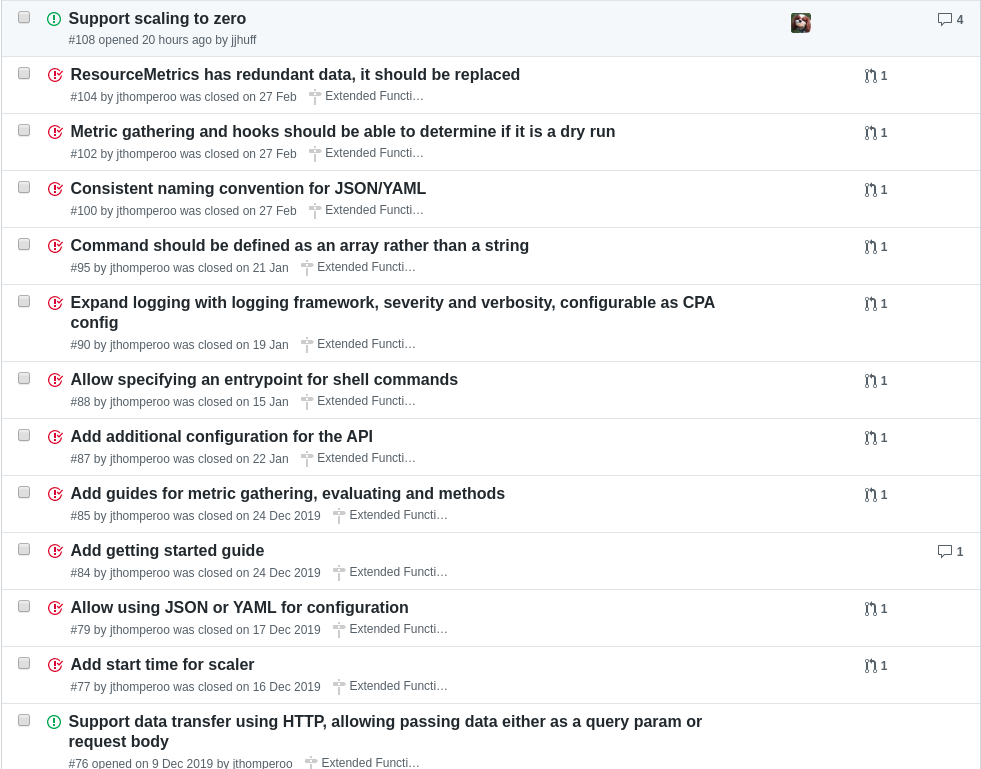
\includegraphics[width=1.0\textwidth]{assets/implementation/gh_issues.png}
\newpage

\subsection*{Appendix F}

Example of a Github Issue.

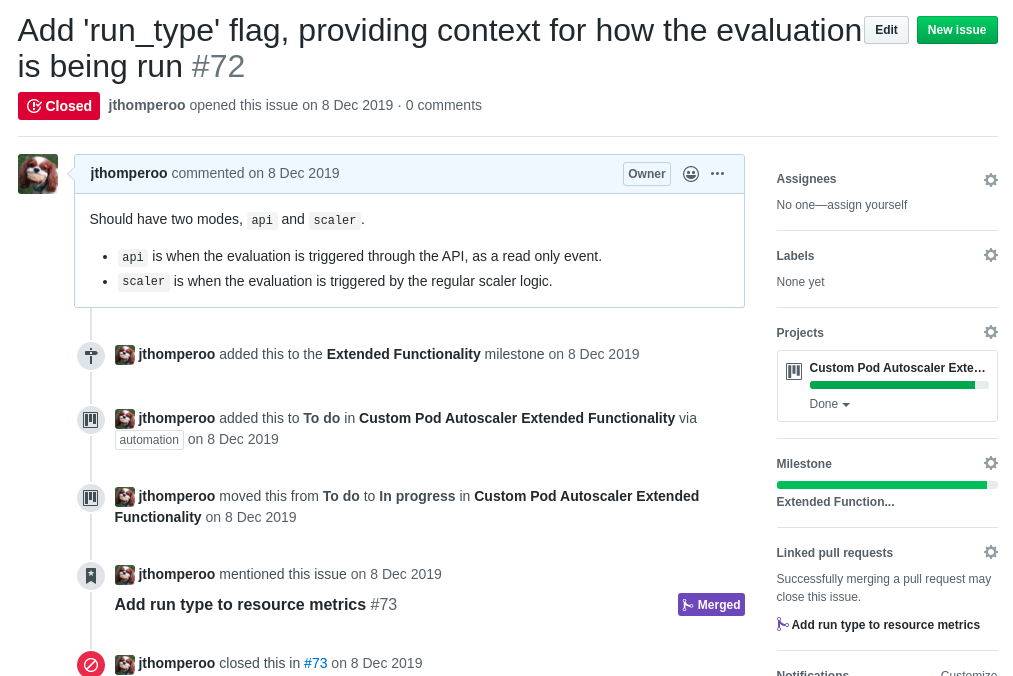
\includegraphics[width=1.0\textwidth]{assets/implementation/gh_issue_example.png}
\newpage

\subsection*{Appendix G}

Example of user feedback through GitHub issue.

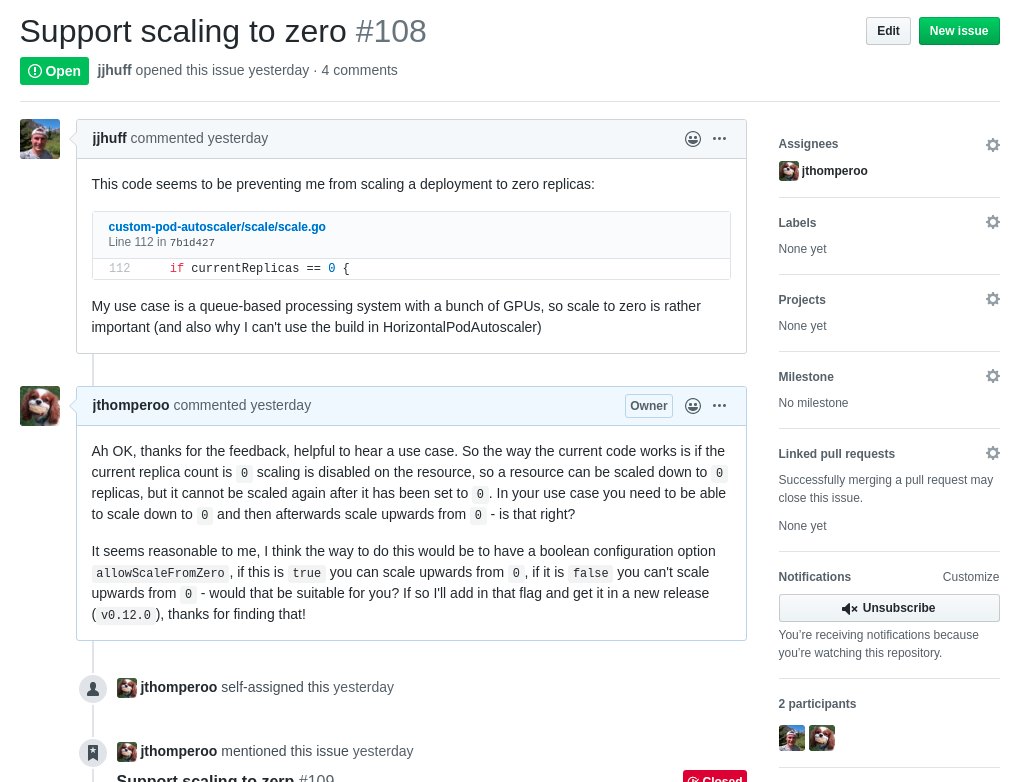
\includegraphics[width=1.0\textwidth]{assets/implementation/user_feedback_issue.png}
\newpage

\subsection*{Appendix H}

Example use case from GitHub issues.

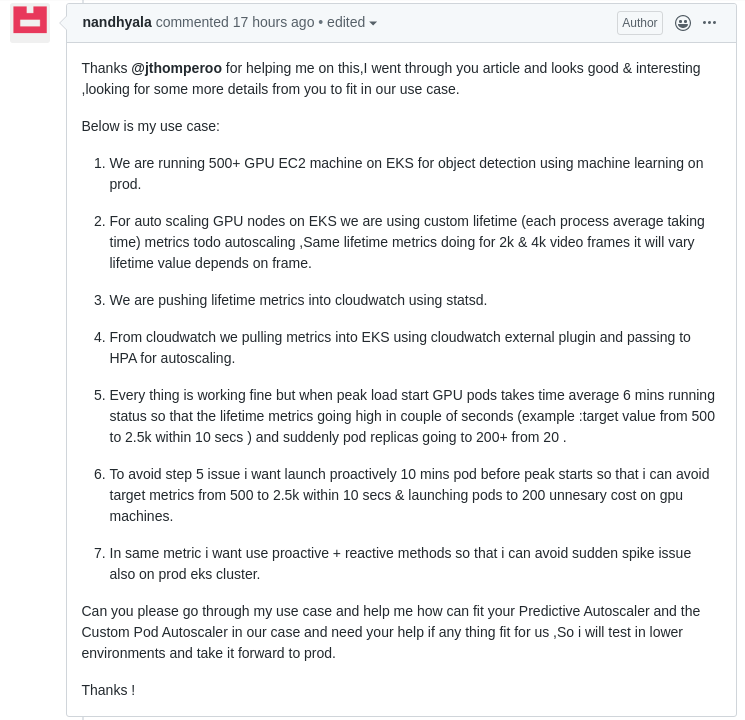
\includegraphics[width=1.0\textwidth]{assets/evaluation/gh_usecase.png}
\newpage
